\chapter{Requirements ESB in Openshift}
\label{cha:esboc}
As discussed in Chapter \ref{cha:esb}, an ESB is a distributed computing architecture, where distributed services act as a consumer or producer. These services provide a business value in form of an integration of an internal or external service for an enterprise. There are multiple providers of ESB middleware like JBoss Fuse, as discussed in Section \ref{sec:esb-middleware}, which provide tooling for implementing service components hosted on an ESB. It should be possible to migrate such a service component to a microservice, where features provided by the ESB middleware will have to be replaced by other implementations.
\\ \\
In this chapter an ESB application will be designed, where a service and a database will be integrated into each other by a another service. An Openshift Project will represent the service bus, which hosts the integration service, provides configuration and manages secrets for it.

\section{Requirements Services}
\label{sec:esboc-design-services}
The service will be implemented in Java with the Java Enterprise Platform and the MicroProfile specifications. The MicroProfile specifications are an effort of the Eclipse Foundation to make Java applications ready for the cloud, where for instance monitoring, logging and tracing are very important aspects to consider when it comes to distributed services. The services will be hosted as standalone applications like Spring Boot applications \cite{EclipseMicroprofileCharter2017, EclipseEE4JCharter2017}.
\\ \\
Each service will run in its own runtime environment and can therefore be deployed independently from the other services. Therefore that each service can be deployed independently, each service must have its own life cycle and source code management. 
\newpage

\begin{figure}[htbp]
	\centering
	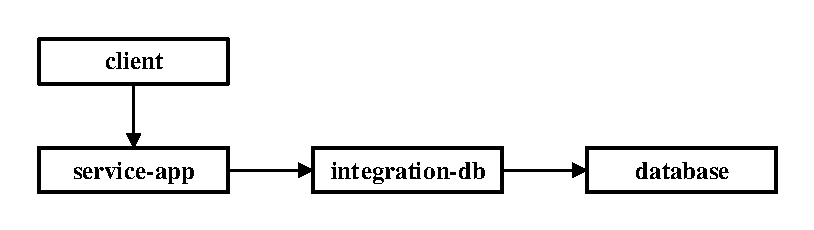
\includegraphics[scale=1]{images/esboc-design-services.pdf}
	\caption{Service Architecture}
	\label{fig:esboc-design-services}
\end{figure} 
The Figure \ref{fig:esboc-design-services} illustrates the services and who they are communicating with. All involved actors except the database will provide their logging and tracing information to a central service for monitoring purposes.

\subsection{Distributed Tracing}
\label{sec:esboc-design-tracing}
Distributed Tracing allows to comprehend service or method call chains. The MicroProfile specifications provides the OpenTracing specification, which provides an API for tracing an application on a method level or across service boundaries. The services must be able to provide tracing information about the REST and the related service call. The tracing implementation must be implemented separately from the service logic  \cite{CNCFOpentracing2018}.

\subsection{Distributed Logging}
\label{sec:esboc-design-logging}
Distributed Logging allows to comprehend information across service boundaries for a specific service call chain. The services must be able to provide all of their logging to a central service and must provide a marker which allows to extract the logs of all related services of a specific service call chain. Optionally the services are allowed to add additional markers.

\subsection{Configuration}
\label{sec:esboc-design-config}
The MicroProfile specifications provide the MicroProfile-Config specification, which provides an API to inject configuration parameters, which can be loaded from different configuration sources. The services must provide the possibility to be configurable for different stages such as DEV (development), TEST (testing) and PROD (productive environment), where the services don't directly access the configuration sources \cite{EclipseMicroprofileConfig2018}.

\subsection{Fault Tolerance}
\label{sec:esboc-design-fault}
The MicroProfile specifications provide the specification MicroProfile-Fault-Tolerance, which provides an API to define fault tolerance behavior such as retries, timeouts and error fallbacks. The fault tolerance of a service means that, if a depending service is not accessible at the time, a service must not fail immediately after the first try, but the service should retry to call the depending service for several times, and fail when all retries have failed. Such a behavior ensures that short timed communication errors, redeployments or overloads do not immediately cause an service to fail. The services must not fail after the first try of an operation, if a other service is involved, but must provide proper fault tolerance configuration to be able to recover from such an error in a proper manner. \cite{EclipseMicroprofileFault2018}.   

\subsection{API Management}
\label{sec:esboc-design-api}
The API management of public API such as REST-API ensures that the clients using an public API are not broken by changes made on the API. There are several opinions on how API management can be done. The services must be capable of migrating their public API in a way that the clients are not broken by the change. The replaced API version must be supported as well as the new one, so that the client is not forced to modify its source code.

\textbf{ADD resource which christoph found during liwestfsw research} 


\section{Requirements Openshift}
\label{sec:esboc-design-oc}

\subsection{Security}
\label{sec:esboc-design-security}
